
\documentclass[12pt]{amsart}
\usepackage{geometry} % see geometry.pdf on how to lay out the page. There's lots.
%\geometry{letter} % or letter or a5paper or ... etc
% \geometry{landscape} % rotated page geometry

% See the ``Article customise'' template for come common customisations
%% LaTeX - Article customise

%%% PACKAGES
\usepackage{booktabs} % for much better looking tables
\usepackage{array} % for better arrays (eg matrices) in maths
\usepackage{paralist} % very flexible & customisable lists (eg. enumerate/itemize, etc.)
\usepackage{verbatim} % adds environment for commenting out blocks of text & for better verbatim
\usepackage{subfigure} % make it possible to include more than one captioned figure/table in a single float
\usepackage{graphicx}

%% END Article customise
\title{hw1 part 2}
\author{Spencer Bliven}

%%% BEGIN DOCUMENT
\begin{document}
\maketitle
\section{Distance functions}

Choosing a distance function is critical for $k$-nearest neighbors. Ideally, the distance function should always return a very small value for points with the same label and very large numbers for points with different labels. The greater the separation between the intra-label and inter-label distributions, the greater the accuracy of the $k$-NN algorithm.  To assess the suitability of various distance functions for image processing, $k$-NN was trained using the USPS zipcode data. The $k$ nearest neighbors, as measured by each distance function, were used to predict the label for each test image. The accuracy of the method is then defined as the percentage of labels correctly predicted.

\begin{table}[htdp]
\begin{center}
\begin{tabular}{llc}
\toprule
\bf{Distance Function} & Formula & \bf{Accuracy} \\
\midrule
Euclidean & $\left( \sum_{i=1}^m (x_i-y_i)^2 \right) ^{1/2}$ &
 94.420\% \\
Weighted Euclidean & $ \left( w_0 + \sum_{i=1}^m w_i (x_i-y_i)^2 \right)^{1/2}$ &
 92.277\% \\
Similarity & $1-\sum_{i=1}^m x'_i y'_i $ &
 94.170\% \\
Weighted Similarity & $1-\left(w_0 + \sum_{i=1}^m w_i x'_i y'_i \right) $ &
 93.274\% \\
Manhattan distance & $ \sum_{i=1}^m | x_i-y_i | $ &
 93.672\% \\
\bottomrule
\end{tabular}
\end{center}
\caption{Accuracy of $k$-NN with a variety of distance functions. Accuracy is measured as the percentage of test points labelled correctly by the algorithm. In each case, $x$ and $y$ represent points in $\mathbb{R}^m$, $w$ represents a weight vector in $\mathbb{R}^{m+1}$. Normalized points are expressed as in $x' = \frac{x}{||x||_2}$. }
\label{tab:distfns}
\end{table}

Five distance functions were considered: Euclidean distance, weighted euclidean distance, similarity, weighted similarity, and manhattan distance. The five functions are summarized in Table~\ref{tab:distfns}, along with the accuracies observed for each.

Euclidean distance (2-norm) and manhattan distance (1-norm) were calculated in the typical manner. Similarity was modified somewhat from the standard dot-product to fit $k$-NN. First, all points were normalized to have norm 1. Next, the similarity was calculated by dot-product, yielding a similarity from -1 to 1. To allow $k$-NN to operate on this function, we took $1-x\cdot y$, yielding a value in $[0,2]$, where lower values indicate closer points.

Weighted euclidean distance and weighted similarity both required training the weights vector, $w$. This was done by minimizing an objective function via linear regression. 
For weighted similarity, the objective function was to minimize
\[ \sum_{j=1}^N \left( \hat{l}_j - w_0 - \sum_{i=1}^m w_i x_i y_i  \right) ^2  + \lambda \sum_{i=1}^m w_i^2 \]
over all $w$, where $\hat{l}_j$ represents the ideal similarity between $x$ and $y$ and $N$ is the number of $(x,y)$ pairs considered during training. In this case, $\hat{l}_j$ is 1 when the labels for $x$ and $y$ match, and -1 otherwise. The USPS training set contains 7291 images. From these, 10000 positive examples of $(x,y)$ with matching labels were chosen at random with replacement, and 20000 negative examples with differing labels were chosen.

   \begin{figure}[htbp]
\begin{center}
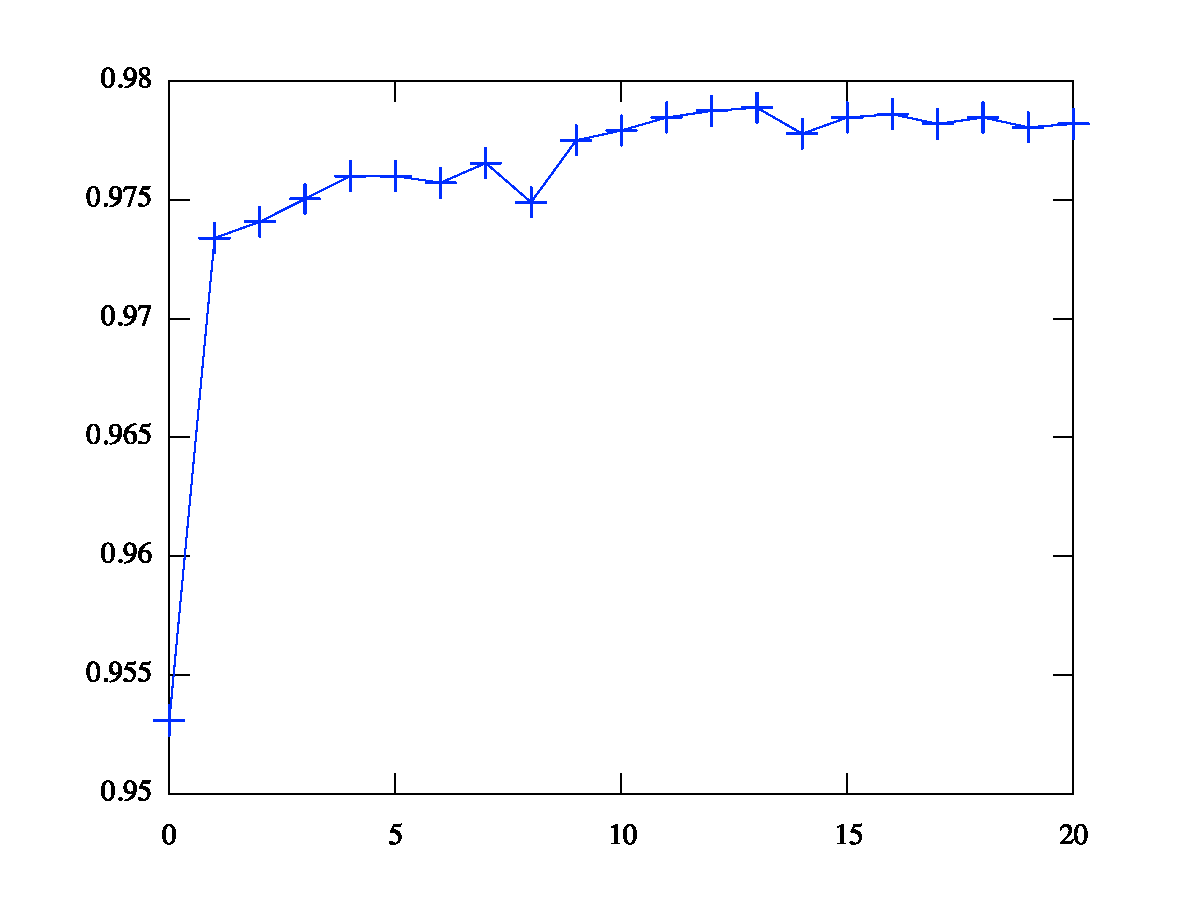
\includegraphics[scale=.5]{weightedSimilarityAccuracy}
\caption{{\bf Accuracy of $k$-NN using weighted similarity with various values of $\lambda$. $\lambda$ is on the x-axis, accuracy on the y-axis.}}
\label{fig:lambda}
\end{center}
\end{figure}


Choosing the penalty coefficient, $\lambda$, is a difficult prospect. A range of values for $\lambda$ were tested, with new weights recalculated for each. Each set of weights was used with $k$-NN to predict labels for the training set (see Figure \ref{fig:lambda}). Using this procedure we found a value of $\lambda=10$ to be optimal. The weights associated with this $\lambda$ were then used to predict the test images.

For weighted euclidean distance, the objective function was to minimize
\[ \sum_{i=1}^N \left( \hat{l}_j - w_0 + \sum_{i=1}^m w_i (x_i-y_i)^2 \right)\]
over all $w$.
Here determining the ideal distance $\hat{l}$ is more difficult. It was chosen to let $\hat{l} = \sum_{i=1}^m (x_i-y_i)^2 $ for negative examples, and $\hat{l}=0$ for positive samples. This attempts to learn weights such that points with the same label will be close, while the distance between unrelated points will be unchanged. 30000 pairs of points were sampled in the same manner as for weighted similarity, and linear regression again used to determine the optimum weights for the objective function.

\section{Lessons Learned}

Of the five distance functions considered, euclidean distance seems to be the best suited for clustering digit images by $k$-NN. However, all distance functions were able to identify digits with high accuracy.

A surprising result is that weighting slightly decreases the accuracy of $k$-NN for both euclidean distance and similarity. For euclidean distance this may be the result of a poor choice of ideal distances. Points with different labels would ideally be infinitely far apart for training, but this is impractical for regression methods. The compromise of using the unweighted euclidean distance as the ideal distance for inter-class pairs appears to have been a poor choice. 

\end{document}